%!TEX root = paper.tex
\section{Methodology}
\label{sec:methodology}


In this section, we propose new techniques to robustly fingerprint all kinds of BLE/bluetooth devices and identify them uniquely in real world setting. According to the two categories of architecture described in the Section~\ref{sec:background}, we design two algorithms to robustly extract the corresponding imperfections. The key insight behind both algorithms is using the entire packet for extracting fingerprints instead of only relying on specific short parts of the packet such as preamble. This gives us the granularity and accuracy which is necessary for device identification task. Finally, we take advantage of both fingerprints to be able to identify any kind of BLE transmitter.
%In order to build a robust algorithm, we would start from the physics of the BLE architectures and build algorithms to capture hardware impariments to uniquely identify each radio. We present a novel algorithm to recover the hardware impairments which WiFi based RF fingerprinting relies on. Specifically, we would discuss how to extract the accurate hardware impairments such as CFO, IQ offset and IQ imbalance with just using the BLE transmissions which have narrow bandwidth with short packet sizes and short preamble length. 

%Next, we un-cover that not all devices use IQ architecture or popular architecture used by WiFi transceivers. In order to reduce power, the  reveal that BLE-only chipsets do not use the commonly known transmitter architecture and consequently, do not have many of the well-known hardware impairments. As a result, we porpose a new technique for profiling those architectures. Finally, we illustrate the overall flow of our fingerpriting methodology.
\begin{comment}
and we show that the second technique can be used to fingerprint any kind of bluetooth transmitter, regardless of the transmitter architecture.
\end{comment}



\subsection{Fingerprinting WiFi/BLE Combo-chips}
\label{sec:methodology1}

%Hardware Impairment estimation for WiFi/BLE Combo-chips}

% Talk about the combo chip first and explain how smartphone use those and therefore we can use the similar hardware impariments as IQ chipsets.

% this sentence says everything in one sentence slow it down, talk about WiFi devices first, show a figure with the architecture of the WiFi chipset to explain

%Practical hardware concerns have made the usage of I/Q path in transmitter architecture including WiFi chipsets, a desirable choice. In this kind of architecture, I and Q data are generated in different paths and eventually they are mixed with the carrier frequency. On the other hand, the hardware imperfections caused by this kind of hardware design, including CFO, IQ offset and IQ imbalance [CITE], have been proposed as important hardware characteristics which can be used to distinguish different devices. Naturally, the devices equiped with both BLE and WiFi technology (e.g. smartphones), utilize the same piece of hardware as a combo chipset for sending both BLE and WiFi packets as shown in Fig. XXXX. The reason lies in cost efficiency, simplifying board design, and optimizing die size and on-board area. As a result, we can take advantage of previously explored hardware imperfections (CFO, IQ offset and IQ imbalance). \\

%In previous works, CFO, IQ offset and IQ imbalance [CITE] have been proposed as important hardware characteristics which can be used to distinguish different devices. 


% Next talk about WiFi decodes the CFO etx and how it does, can we apply similar technique to BLE, we cannot, why?
% talk about how BLE is challenging with narrow bandwidth, short preamble makes it hard to detect CFO, if similar techqnieu as WiFi is applied what is the resolution you would get and would it resolve the devices (make the problem look hard)

%Measuring these harware imperfections is an unavoidable stage in decoding WiFi packets since it can significantly affect the decoding error if the receiver does not compensate them. As a result, measuring these imperfection has been heavily researched for WiFi signals. More than that, pecific arrangements have been devised in WiFi protocol to make the estimation of these imperfections easy and accurate. On the other hand, decoding the simple GFSK modulation which is used in BLE and Bluetooth, is not affected by the aforementioned imperfections severly. Therefore, there has not been any attempt on measuring these impairments accurately for a BLE or Bluetooth signal. Also, using the same techniques for estimating impairments as WiFi, will result in a much lower accuracy of estimation because of having a narrowband (without subcarrier) short signal (typically a few hundreds of microseconds) with a very short premble (8 microseconds). For instance, we employed the technique that is used in Bluetooth test equipments which exploits the preamble to estimate CFO [CITE]. That is, simply we take the average of frequencies in the preamble. Since preamble is an 8-bit sequence of consecutive 0 and 1, the frequency of preamble is symmetric. Therefore, ideally the average of thh frequencies in preamble must be 0. If there exists CFO, this average will be an estimate of CFO. However, this estimation is not precise and robust as it only relies on a an 8-microsecond preamble. The resulting standard deviation of the measured CFO was 1.5 KHz (we averaged the CFO standard deviation across 20 different devices). This standard deviation is huge for performing the task of RF fingeprinting and will end up in low accuracy of identifying devices based on RF fingerprints. We also tried the MINMAX algorithm described in [CITE] but it yields even worse standard deviation.\\

% then propose your solution layer by layer, first layer to increase the resolution your idea is to use entire packet, which requires you to decode the data and then reconstruct the receive singal witout hardware impariment and use that to estimate the impariements. 

As discussed in Section~\ref{sec:background}, CFO, IQ offset and IQ imbalance are important hardware characteristics that can be leveraged to uniquely identify this kind of architecture as proposed by prior works for fingerprinting WiFi devices as well. However, the challenge is how we can estimate these imperfection parameters accurately and fine-grained to fulfill the device identification task. WiFi signal eases this job by having specific signal features such as LTF and multiple subcarriers (and also WiFi chipsets report CSI which can easily be used to estimate these imperfections). This is mainly because fine-grained estimation and compensation of CFO and IQ imperfections is an unavoidable step in decoding WiFi signal. If CFO compensation is not accurate in WiFi decoding, IQ samples will rotate by time, and if IQ imperfection is not compensated, the shape of constellation will change. Both of these will drastically affect the decoding process since symbols are modulated in IQ domain. As a result, the mentioned signal features have been anticipated and there is a huge body of work on how to etimate these imperfections accurately for WiFi signals (not only for RF fingeprinting, but also for other purposes).


On the other hand, decoding BLE or Bluetooth signals is not affected by CFO and IQ imperfections. In fact, even several KHz of CFO will not affect the decoding process of GFSK signals and since symbols are not modulated in IQ domain, IQ imperfection does not affect BLE decoding process. As a result, unlike WiFi, there was no need to embed any signal feature in BLE signal to provide necessary means for accurate and fine-grained etimation of these imperfections. For instance, BLE preamble is only 8 bits (8 microseconds) which is much shorter than WiFi, it uses the simple GFSK modulation, and there does not exists multiple subcarrier in BLE signal or CSI in BLE chipsets. These simplicities of BLE signal leaves us in a situation where estimating these imperfections for BLE signals is much more challenging than WiFi. The consequence of this fact is that existing techniques for fine-grained estimation of CFO and IQ imperfection of WiFi signals, either cannot be adopted or will not result in fine-grained imperfection estimation for BLE signals. Moreover, techniques that are specifically designed for CFO estimation of BLE or Bluetooth signals provides only a very coarse-grained estimation which is not sufficient for device identification task at all, and not surprisingly, there has not been any attempt on estimating IQ imperfection for BLE or BLuetooth signals as it is not needed for decoding. In fact, no prior work has demonstrated that it is possible to obtain accurate and identifiable estimates of imperfections for BLE transmitters. Consequently, we must develop a new algorithm to enable find-grained and robust CFO and IQ imperfections to enable our device identification attack.

In fact, the most accurate existing technique for BLE or Bluetooth CFO estimation that we found is the technique that is used in Bluetooth test equipments which exploits the preamble to estimate CFO~\cite{}. That is, simply we take the average of frequencies in the preamble. Since preamble is an 8-bit sequence of consecutive 0 and 1, the frequency of preamble is symmetric. Therefore, ideally the average of the frequencies in preamble must be 0. If there exists CFO, this average will be an estimate of CFO. However, this estimation is not precise and robust enough as it only relies on a an 8-microsecond preamble. We further extended this method to take advantage of the entire packet and take average across frequencies of equal number of 0's and 1's. However, we did not see any significant benefit for doing that. Another popular algorithm for BLE/Bluetooth CFO estimation is the MinMax algorithm. We refer the readers to~\cite{} for the explanation of this algorithm. To demonstrate that none of these techniques are accurate and fine-grained enough for the task of identification, we take 40 BLE devices and compute CFO using all 3 aforementioned existing techniques (averaging preamble, its extension and MinMax) for 100 packets for each. For eeach device, we consider the technique which yielded the lowest standard deviation (std). Figure~\ref{fig:cfo_comp} shows the interval $[mean-std,mean+std]$ of CFO for these 40 devices (gray bars). Clearly, many of these 40 devices are confused if the existing CFO estimation techniques are employed. Hence, we need to develop a new technique for fine-grained and accurate CFO estimation to enable device identification. Figure~\ref{fig:cfo_comp} also shows the same interval when using our proposed imperfection estimation technique (blue bars). With the significantly reduced standard deviation for all devices, these 40 devices are now much more separable.

\begin{figure}[t!]
    \centering
    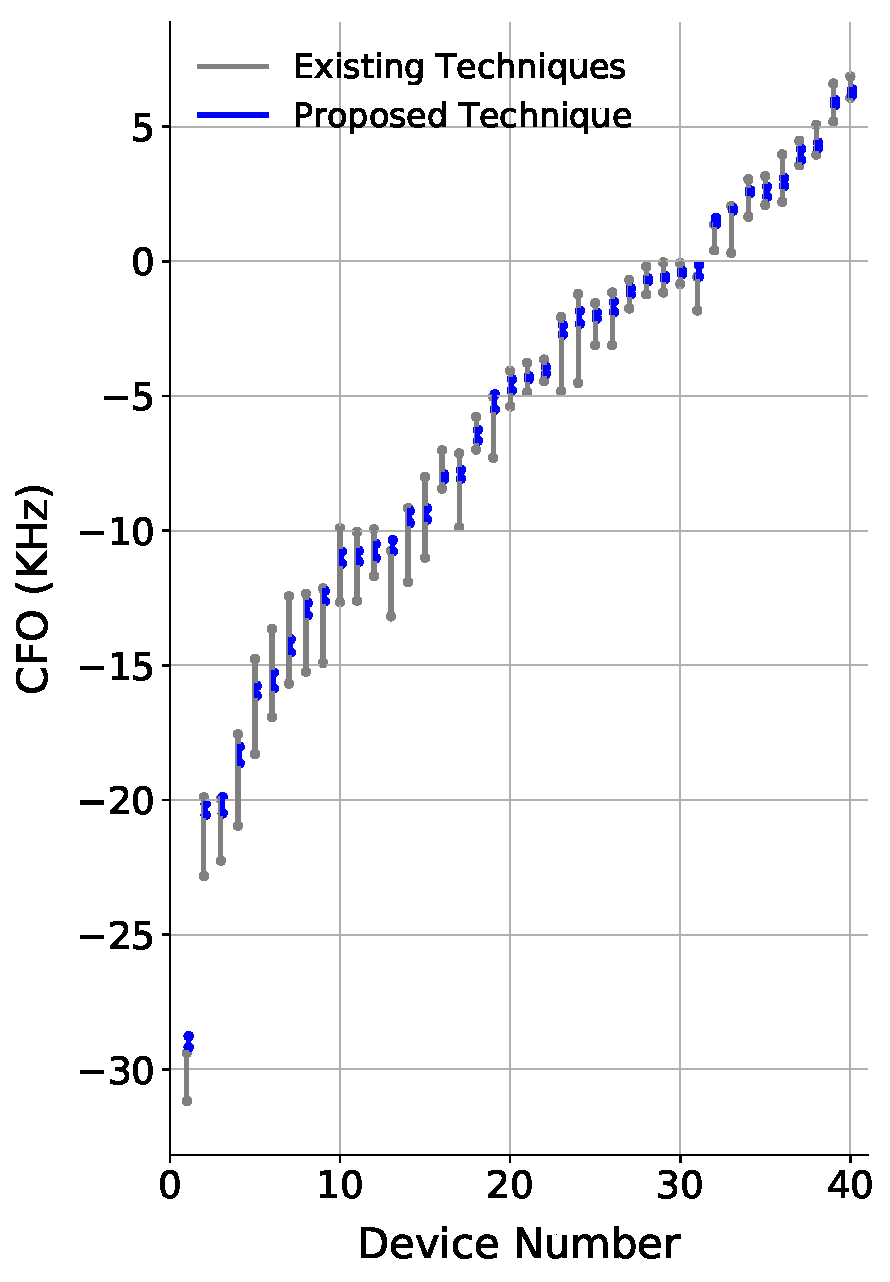
\includegraphics[width = \linewidth]{plots/CFO_comparison.pdf} 
    \caption{Comparing the CFO estimation of existing techniques with our proposed technique - While BLE CFO estimation using existing techniques results in lots of confusion between devices, our proposed technique significantly increases within class variance for a device which is necessary for identification task}
    \label{fig:cfo_comp}
\end{figure}
%The resulting standard deviation of the measured CFO was 1.5 KHz (we averaged the CFO standard deviation across 20 different devices). This standard deviation is huge for performing the task of RF fingeprinting and will end up in low accuracy of identifying devices based on RF fingerprints. 

Moreover, inaccurate estimation and compensation of CFO affects the estimation of IQ imperfections since the residual CFO will cause IQ samples to rotate by time. These facts and observations suggests that the suitable algorithm for BLE imperfection estimation must have two key properties. First, instead of relying on preamble (or any other specific short parts of the packet), it must utilize the entire packet in order to diminish the effect of noise and provide more information and granularity for accurate imperfection estimation. Second, CFO and IQ imperfections must be estimated jointly and with high granularity to prevent the mutual effects on each other's estimation. Keeping these two key properties in mind, we develop an algorithm to estimate CFO and IQ imperfections for BLE signals.

To be able to take advantage of the entire packet properly, we need to first decode the packet. Note that thanks to simple GFSK modulation, hardware imperfection does not cause decoding error as opposed to WiFi. Therefore, decoding can be done properly without compensating hardware imperfections. Once we have the decoded data, we can reconstruct the ideal signal. The high level idea is that we insert hardware imperfection parameters in the mathematical model of the ideal signal. Then we keep changing those imperfection parameters until the mathematical representation of the signal looks like the actual captured signal. However, since the search space for these imperfection parameters is vast, we use optimization techniques to move towards the optimal value of parameters efficiently.

%However, to build an algorithm for estimating these fingerprints accurately and robustly, despite the existing techniques, we cannot rely on the preamble since it is very short for BLE and also, there is no notion of subcarrier in BLE technology. For instance, we employed the technique that is used in Bluetooth test equipments which exploits the preamble to estimate CFO~\cite{?}. That is, simply we take the average of frequencies in the preamble. Since preamble is an 8-bit sequence of consecutive 0 and 1, the frequency of preamble is symmetric. Therefore, ideally the average of the frequencies in preamble must be 0. If there exists CFO, this average will be an estimate of CFO. However, this estimation is not precise and robust enough as it only relies on a an 8-microsecond preamble. The resulting standard deviation of the measured CFO was 1.5 KHz (we averaged the CFO standard deviation across 20 different devices). This standard deviation is huge for performing the task of RF fingeprinting and will end up in low accuracy of identifying devices based on RF fingerprints. \\

%Instead of relying on preamble or specific short parts of the packet, we can benefit from the entire packet to make a robust and accurate imperfection estimator since using the entire packet helps in diminishing the effect of noise as well as providing more information and granularity to estimate imperfections accurately. Although for being able to take advantage of the entire packet properly, we need to first decode the packet. Note that thanks to simple GFSK modulation, hardware imperfection does not cause decoding error as opposed to WiFi. Therefore, decoding can be done properly without compensating hardware imperfections. Once we have the decoded data, we can reconstruct the ideal signal. The high level idea is that we insert hardware imperfection parameters in the mathematical model of the ideal signal. Then we keep changing those imperfection parameters until the mathematical representation of the signal looks like the actual captured signal. However, since the search space for these imperfection parameters is vast, we use optimization techniques to move towards the optimal value of parameters efficiently. \\
%Although we consider GFSK modulation in this paper, the idea behind this method can be extended to many other modulation schemes. 

% estimating impariments is not easy, explain the math model and explain why it is hard, as it not convex 

% present your insights to use a gradient descent algorithm, however even that gets stuck at local minima's which is not great, so you fix this by choosing right intial value. 

% explain how you choose right initial value, what are your insgihts and why does those work. 

% finally show the performance of your algorithm before ending the section. 




\begin{comment}
    To measure these hardware impairments, we mathematically model them and then use optimization techniques to estimate these imperfections. 
\end{comment}
Let $y = Real\{y\}+jImag\{y\}$ be the captured baseband signal (normalized by the average amplitude). In a GFSK modulated signal, ideally we have $Real\{y\} = cos(\omega(t)t)$ and $Imag\{x\} = sin(\omega(t)t)$ where $\omega(t)$ is the baseband frequency of the signal which is generated according to the GFSK modulation. However, the aforementioned hardware imperfections will slightly change the signal. We first decode the signal to obtain the sequence of bits and then, we make $\omega(t)$ according to GFSK modulation. Let $y'$ be the model of the imperfect signal. Considering the effects of CFO, IQ offset and IQ imbalance, we can write
\begin{gather*}
    y'(t) = \big[(A-\frac{\epsilon}{2})cos(\omega(t)t-\frac{\phi}{2})+I+ \\
    j\big((A+\frac{\epsilon}{2})cos(\omega(t)t+\frac{\phi}{2})+Q)\big)\big]e^{j(\phi_o+2\pi f_o t)}
\end{gather*}
where $f_o$, $\phi_o$, $A$, $\frac{\epsilon}{A}$, $\phi$, $\frac{I}{A}$ and $\frac{Q}{A}$ denote CFO, phase offset, normalized amplitude of the signal, IQ amplitude imbalance, IQ phase imbalance, I offset and Q offset, respectively. The goal is to choose the value of these variables in such a way that $||y'-y||^2$ is minimum and as a result, $y'$ is as close as possible to the captured signal $y$. Therefore, we must solve the following optimization problem:
\begin{gather*}
    min_{f_o,\phi_o,A,\epsilon,\phi,I,Q}{F=||y'-y||^2 =} \\ |Real\{y'\}-Real\{y\}|^2+|Imag\{y'\}-Imag\{y\}|^2
\end{gather*}
However, this problem is not convex. Consequently, any optimization technique may end up in a local optima. To avoid this, we initialize the variables properly to increase the chance of finding the global minimum significantly. Although theoretically it will not guarantee ending up in the global minimum for arbitrary optimum numbers of these variables, we found that in practice we will reach the optimum value with this initialization in practical conditions. 

To initialize CFO, we take the average of frequencies in the preamble as explained above~\cite{?}. Then we compensate the initial CFO in the signal to get the signal $z = y e^{-2\pi f_o t}$. To estimate initial I/Q imperfections, we use the I/Q constellation of the GFSK signal. The I/Q constellation of an ideal GFSK signal is a circle centered at $(0,0)$ since the phase changes according to GFSK modulation but the amplitude is always constant. However, I/Q imperfection will change this constellation. Speciffically, I/Q offset will shift the center of the circle as it is equivalent to adding a fixed complex term to the ideal signal, and IQ imbalance will change the shape from a circle to a tilted ellipse. These effects are shown in Figure~\ref{fig:iq_const}. As a result, to get an initial estimation of IQ imperfections, we fit an ellipse to the 2-dimensional points $(Imag\{z\},Real\{z\})$ by minimizing the Least Square Error. The center of the ellipse will provide the initial IQ offset and initial IQ imbalance can be obtained from the ratio of minor and major diameter and rotation angle of the ellipse.\\
\begin{figure}[t!]
    \centering
    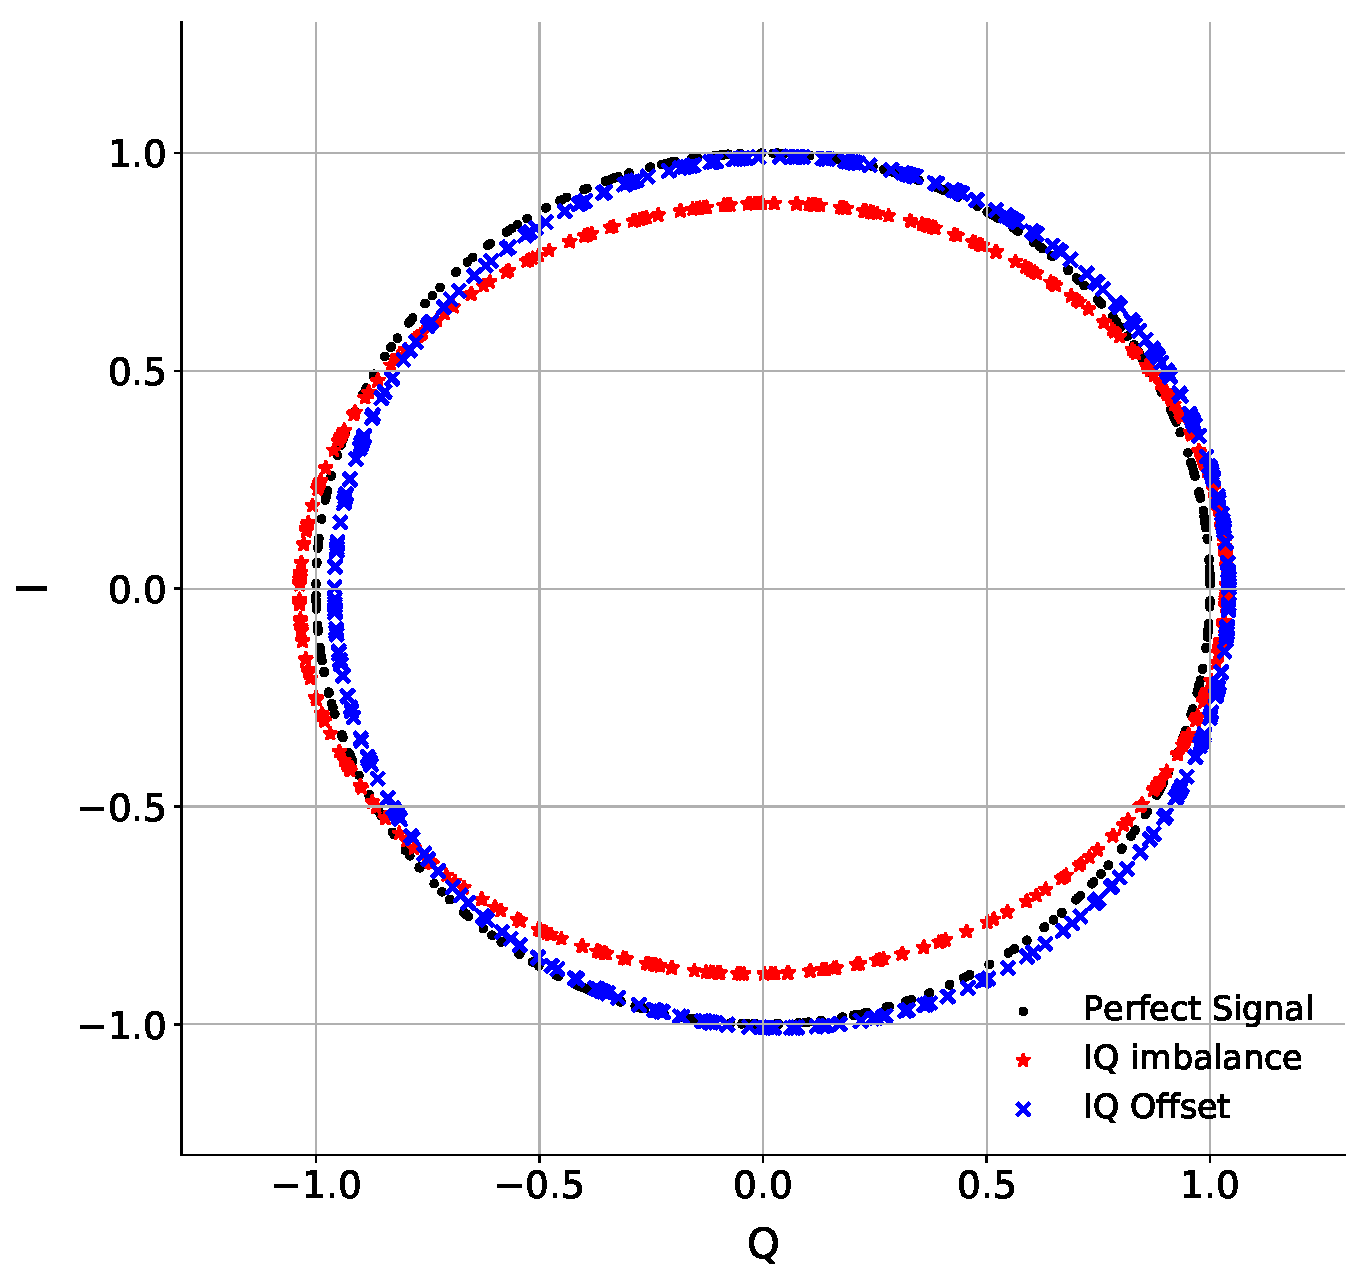
\includegraphics[width = \linewidth]{plots/IQ_const.pdf} 
    \caption{Effects of IQ imperfection on IQ constellationo of a GFSK signal without noise and CFO}
    \label{fig:iq_const}
\end{figure}
%it will be long if I want to explain this ellipse thing

Although, these initial estimations provide an initialization close to optimum, they are not precise enough. As mentioned earlier, this initialization of CFO is not precise and robust enough as it only relies on an 8-microsecond preamble. Also, mismatch in CFO compensation will cause a time-dependent phase shift which distorts the I/Q constellation. Therefore, the initial IQ offset and imbalance estimation will also have errors. Consequently, we employ optimization techniques to jointly estimate hardware imperfection parameters precisely and robustly. Therefore, after this initialization, we use Nesterov Accelerated Gradient Descent (NAG)~\cite{?} to move towards the optimum values of $f_o,\phi_o,A,\epsilon,\phi,I,Q$ by minimizing $F$ in the mentioned optimization problem.

However, as mentioned earlier, this optimization problem is convex and we may converge to the local optima. Therefore, if after convergence, the average of $F$ was not less than a certain threshold which is determined according to SNR, we add certain steps to the first initialization and repeat the aforementioned gradients descent process. We keep searching for the optimum with new initializations until either the average of $F$ falls below the threshold or our initialization falls out of the bound of the typical values for these imperfections (in which case we give up on the packet. This typically happens when the SNR is less than 5 dB or there is a collision). The first initialization will increase the speed of convergence as usually it will be close to the optimum and re-initialization will ensure ending up in a point which is either the global optimum or very close to global optimum (in the sense that the objective function is less than the desired threshold and hence, is within a small margin of global optimum). The proposed algorithm fulfills the two key properties that we explained at the beginning of this subsection. First, the NAG based joint estimation of CFO and IQ imperfections ensures precise estimation with fine granularity as it keeps moving towards the optimum with adaptive steps and removes the mutual effect of mismatch in estimating these imperfection parameters. Second, the objective function of optimization is chosen as the summation of all PHY samples across the packet, which diminishes the impact of AWGN and provide more robust information and granularity. The final result is achievement of a highly precise CFO and IQ estimates for a device, that are robust to environmental noise, and can therefore be used by an attacker as a unique fingerprint for generic consumer devices.


We use this methods to extract CFO, IQ offset and IQ imbalance for 20 ESP32 chipsets of the same make and model. Figure~\ref{fig:esp} represents CFO and IQ offset magnitude for 10 packets for each of these 20 chipsets. The low variance of CFO for each device, shows this methods is very precise in measuring hardware imperfections (e.g. the CFO standard deviation average for 20 devices is 200 Hz in our algorithm which is significanly less than the existing methods described earlier). Obviously, low within-class variance will significantly improve the identification accuracy and these 20 devices can be clearly distinguished only by their CFO and IQ offset. \textit{In summary, for the first time we showed that it is feasible to estimate CFO and IQ imperfections of WiFi/BLE combo chipsets based on the simple BLE signal itself; in other words, without needing the rich signal features that are present in WiFi.}




\subsection{Fingerprinting BLE-only chipsets}%Universal Algorithm for all Low Power BLE Architecture }
%we should change the title
\label{sec:methodology2}
%\todo{[add a photo of architecture]}


Next, we employ the same method to extract CFO, IQ offset and IQ imbalance for 20 BLE-only (TI CC2640) chipsets of the same make and model. Figure~\ref{fig:ti} represents CFO and IQ offset magnitude for 10 packets for each of these 20 chipsets. Unlike, ESP32 chipsets, there is no IQ offset in TI BLE boards and we are just left with CFO as a hardware imperfection. As explained in section~\ref{sec:background}, the reason is in low power BLE-only architecture, there is no I and Q paths. Clearly, many of these devices are confused by just using CFO as an RF fingerprint. 
%Furthermore, we used the transient portion of the signal as RF fingerprint, however, even that turns out to be not sufficient for distinguishing devices because it is a very short portion of the signal~\cite{?}. 
However, as explained in Section~\ref{sec:background}, the imperfections in the analog parts of the PLL could potentially be a rich source for distinguishing different devices. This imperfection in low power devices has never been studied as an RF fingerprint before. \textit{Therefore, we propose a technique which is the first to demonstrate there are features in the signals from the low-power design used in BLE-only transmitters which can be employed to uniquely identify the devices.} Next, we will show that the effects of environmental conditions on the proposed method is insignificant, and and explain how our method can make the machine learning models robust to the noise.




%In fact, unlike the combo chipsets, these BLE-only chipsets utilize a fundamentally different architecture without I/Q paths and mixer as shown in Fig. XXXXX. In such architecture, the modulated samples are directly fed to a Phase-Locked Loop (PLL) which generates the required frequencies by moving the carrier frequency up and down. There exist different designs for such an architecture. For instance, in some of them, the loop will be opened once the channel frequency is fixed and the GFSK frequencies are generated in an open-loop VCO [CITE]. In some other, digital modulated samples drive a DCO which adjusts the frequency using capacitors and a $\Sigma \Delta$ modulator. In all these designs, unlike the former architecture in which I/Q imbalance and I/Q could be useful features for fingerprinting devices, there is no I/Q in the RF chain. Instead, the imperfections in the PLL could be a rich source for distinguishing different devices. Depending on the design, these imperfections could have different sources such as loop filter, VCO, capacitors,etc. However, the key fact about these kind of imperfections is that, no matter what is the source, it will represents its effect in the frequencies generated by the transmitter since PLL is responsible for outputing the frequeency of GFSK signal. As a result, to take advantage of this new source of imperfection, we must profile the frequencies generated by the transmitter. 

%The immediate solution for profiling frequency, is using Fourier transform. However, there is a major problem with using Fourier transform. BLE advertisements sent by a device, quite often have a fixed payload data (or at most a very small set of different payload data). As a result, during a MAC address lifetime, the whitened packet sent from a device is fixed. Consequently, we found that if we train a machine learning model on the signal or Fourier transform of the signal, it will simply ignore extracting those slight hardware imperfections since it can simply distinguish devices by only using their packet bit sequence. However, in the next MAC address lifetime, the change in MAC address (and possibly other parts of the payload) completely changes the packet after whitening. Consequently, we cannot identify the device anymore because instead of any hardware imperfections, it has just learnt to distinguish the devices based on their packet sequence. Thus, using Fourier transform does not work for our problem. Therefore, we propose a technique which profiles frequencies generated by a transmitter without preserving any other information that biases the learning model. 

\begin{comment}
As both kind of architecture are commonly used in different BLE devices, any fingerprinting technique that is used should be able to profile both aforementioned characteristics properly regardless of the kind of architecture that is used in the BLE device.\\
\end{comment}

\begin{comment}
As mentioned in sections 2.5 and 3, none of the previous works is sufficient to fingerprint the behaviour of PLL. Therefore, we propose a technique which is suitable to do so. In section 3.4 we will theoretically argue about the effects of environmental conditions on the proposed method and explain how this method can make the job of machine learning models easier in terms of dealing with noise. 
As both kind of architecture are commonly used in different BLE devices, eventually we combine both techniques to be able to fingerprint any kind of BLE transmitter.\\
\end{comment}

\begin{comment}
As some of the BLE transmitters use the aforementioned low power architecture and some other employ the traditional IQ modulation, our proposed technique must include imperfection information of both kind of hardware in order to be a universal solution for identifying BLE devices. Although we could use our gradient descent technique for I/Q-based transmitters and the new technique for PLL-based transmitters, the fingerprinting technique will be less complex if we could use only one of the techniques for any kind of device (add other reasons why universality is good). Thus, in section 4.5, we show how different hardware imperfections present themselves in the proposed method. After that, we will discuss the choice of classifier for classifying devices. One can extend the general philosophy behind our methodology to other wireless communication technologies and modulations.
\end{comment}


\begin{figure}[t!]
    \centering
    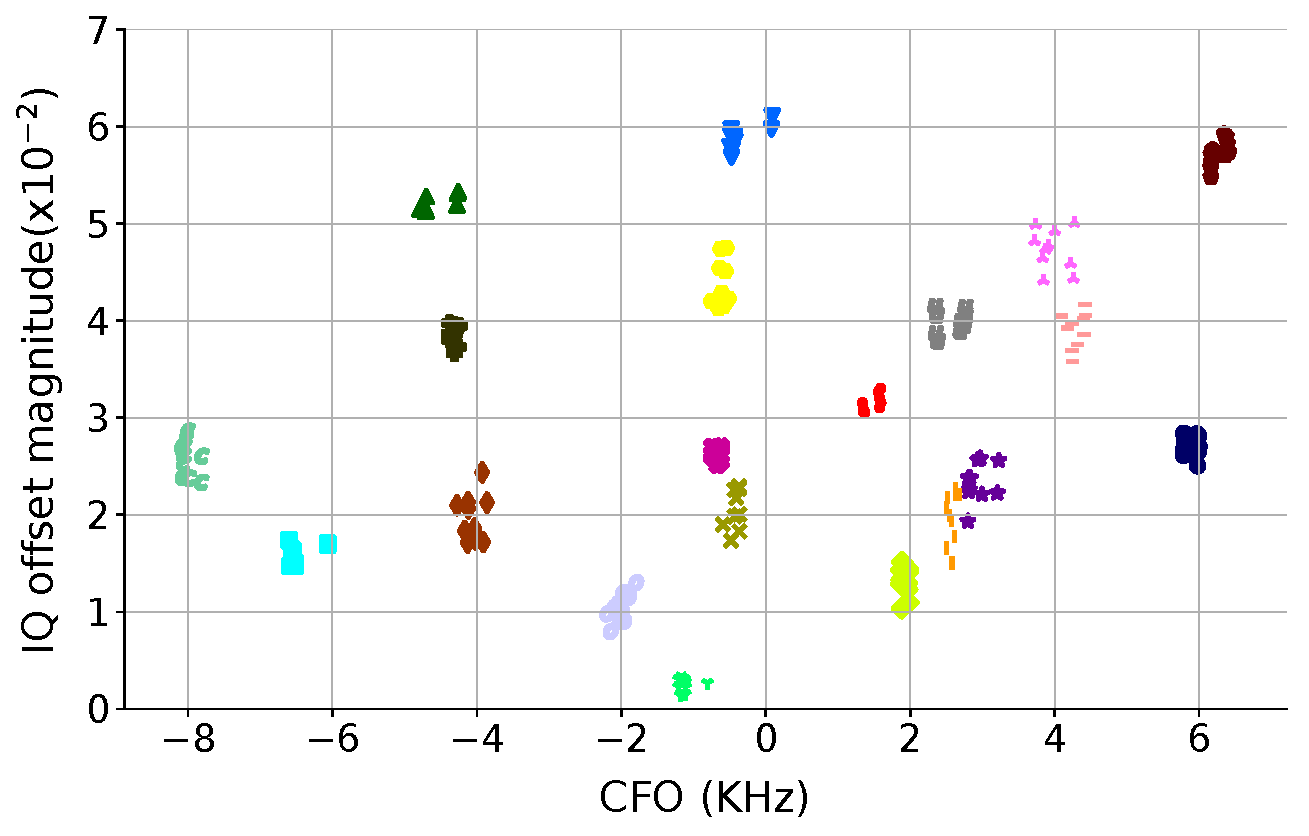
\includegraphics[width = \linewidth]{plots/ESP_CFOIQ.pdf} 
    \caption{CFO and IQ offset magnitude for 20 ESP32 chipsets}
    \label{fig:esp}
\end{figure}

\begin{figure}[t!]
    \centering
    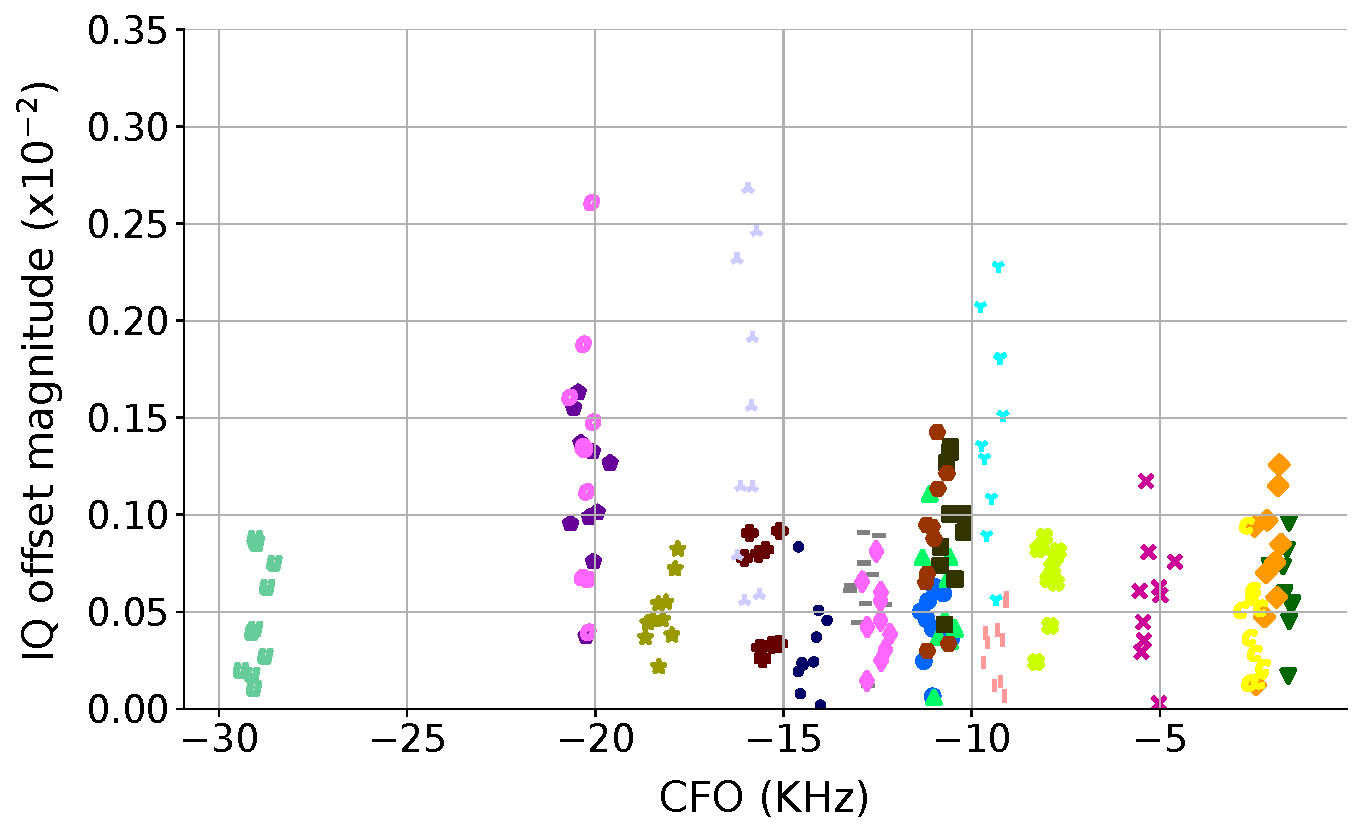
\includegraphics[width = \linewidth]{plots/TI_CFOIQ.pdf} 
    \caption{CFO and IQ offset magnitude for 20 CC2640 BLE chipsets}
    \label{fig:ti}
\end{figure}



\subsubsection{PLL Profiling using Frequency Distribution}
%Since PLL is responsible for generating the frequency of GFSK signal, we must profile the frequencies generated by the transmitter. %However, we cannot employ Fourier transform to profile the generated frequency as discussed in Section~\ref{sec:background}. 
%Therefore, First, we propose a technique which profiles frequencies generated by a transmitter which can preserve all the information that could profile PLL's. 

In BLE-only chip design, since PLL generates the instantaneous frequency of the GFSK signal, imperfections in PLL will manifest itself in the generated instantaneous frequency. Therefore, to profile this imperfections, our key insight is to obtain instantaneous frequency from the received signal. The instantaneous frequency can be obtained by taking the derivative of phase, between two consecutive samples.  Therefore, in order to obtain the instantaneous frequency of the received packet, we take the numerical derivative of the phase of the consecutive samples as follows:
\begin{equation}
\centering
    2\pi f_t = \frac{\phi(t+h)-\phi(t-h)}{2h} \rightarrow f_t = \frac{\phi(t+h)-\phi(t-h)}{4h\pi}
\end{equation}
where $h = \frac{1}{f_s}$ and $f_s$ is the sampling rate of the receiver. Furthermore, we aim to take advantage of the entire packet instead of relying only on specific parts of the packet such as preamble or transient part so that we can build a more robust fingerprint for the devices.
%The instantaneous frequency of a typical GFSK modulation is shown in Fig. \ref{fig:1}. 

However, the instantaneous frequency itself preserves the information about the pattern of bits which can lead to overfitting. This particularly happens because BLE advertisements transmitted from a device usually have the same payload (and therefore, the same pattern of bits) during one MAC address lifetime and when MAC address changes, the payload changes too. As a result, during training, the ML model will just need to learn that bit pattern (or a very few different bit patterns for one device) to be able to identify a device instead of learning any slight hardware imperfections since this is the same for a device during a MAC address lifetime but different for different devices. However, when the MAC address changes and we want to identify the devices, the ML model won't be able to do so as it has only learned the pattern of bits for each device. Consequently, we have to represent the instantaneous frequency in a way which is not dependent of these bit patterns while keeping the necessary information the PLL imperfections.
%However, the instantaneous frequency itself preserves the information on a particular sample of the packet as well. Ideally, we would like to eliminate the information on a particular sample and only observe the PLL's behavior. We mitigate this problem by computing a statistical representation of the frequency profile across the entire packet, so that not only it preserves all imperfection information in the output frequency of PLL, and ignores the information in the samples of the received signal.

% which simply means the instantaneous frequency of two different packets are completely different and dependent on the order of bits. We found it is very common in a typical device like a smartphone that the beacons in one time slot are all the same and as the MAC address changes, the packet changes drastically due to whitening. As we have to use one time slot with a fixed MAC address for training the learning model and classify the devices when their change their MAC address, in many situations we will have only 1 packet during the training and we have to test on a completely different packet. Therefore, any input that we use for training the learning model should be completely robust to bit ordering of the packet in order not to overfit the packet pattern instead of learning subtle hardware imperfections. The reason behind the fact that we do not use Discrete Fourier Transform (DFT) on the entire packet to obtain the frequency components, originates from the same insight. 

The key insight behind the idea is that any hardware characteristic of the device will constantly show itself across the packet. As a result, the distribution of the frequency values measured across the packet will have the information about hardware imperfection that are robust enough to be used for fingerprinting the device. We call such a distribution as "Frequency Distribution". Although frequency distribution is not dependent on bit ordering, it is dependent on the relative number of bit 0 and bit 1. Due to packet whitening, the number of 0 bits and 1 bits will be approximately the same. However, to remove the slight biases and get the best performance, we take equal number of 0 and 1 bits aftre decoding and discard the rest of the bits.

%Furthermore, as we take advantage of the entire packet instead of relying only on specific parts of the packet such as preamble or transient part, we can build a more robust fingerprint for the devices. The key insight behind the idea is that any hardware characteristic of the device will constantly show itself across the packet. As a result, the distribution of the frequency values measured across the packet will have the information about hardware imperfection that are robust enough to be used for fingerprinting the device. We call such a distribution as "Frequency Distribution". Although frequency distribution is not dependent on bit ordering, it is dependent on the relative number of bit 0 and bit 1. Due to packet whitening, the number of 0 bits and 1 bits will be approximately the same. However, to remove the slight biases and get the best performance, we take equal number of 0 and 1 bits and discard the rest of the bits. \\

To represent the frequency distribution of the received signal, we bin the measured frequency values, assign each frequency to the corresponding bin, calculate the total number of frequency measures in each bin, and and call the resulting array a Histogram. Binning simply means that we divide the frequency range of $[-f,f]$ to $\frac{2f}{f_b}$ bins, each of which has the size of $f_b$. The choice of bin size $f_b$ is made experimentally. Finally, we normalize the Histogram so that all bin counts add up to 1, similar to a distribution. A sample of the histogram for 3 different CC2640 BLE chipsets is shown in Figure~\ref{fig:3}. For each transmitter, we averaged the Histogram across 10 packets to avoid the changes because of environment so that the figure only represents the actual differences due to hardware imperfections. The two global maximas represents $\pm f_d$, the frequencies corresponding to 0 and 1 bits and the two smaller peaks represent the situation in which we have '010' and '101' sequences and the frequency cannot reach the exact $\pm f_d$ value for the middle bit due to the Gaussian transition. 
%All other bin elements represent the Gaussian transitions between 0 and 1 bits.

\begin{figure}[t!]
\centering
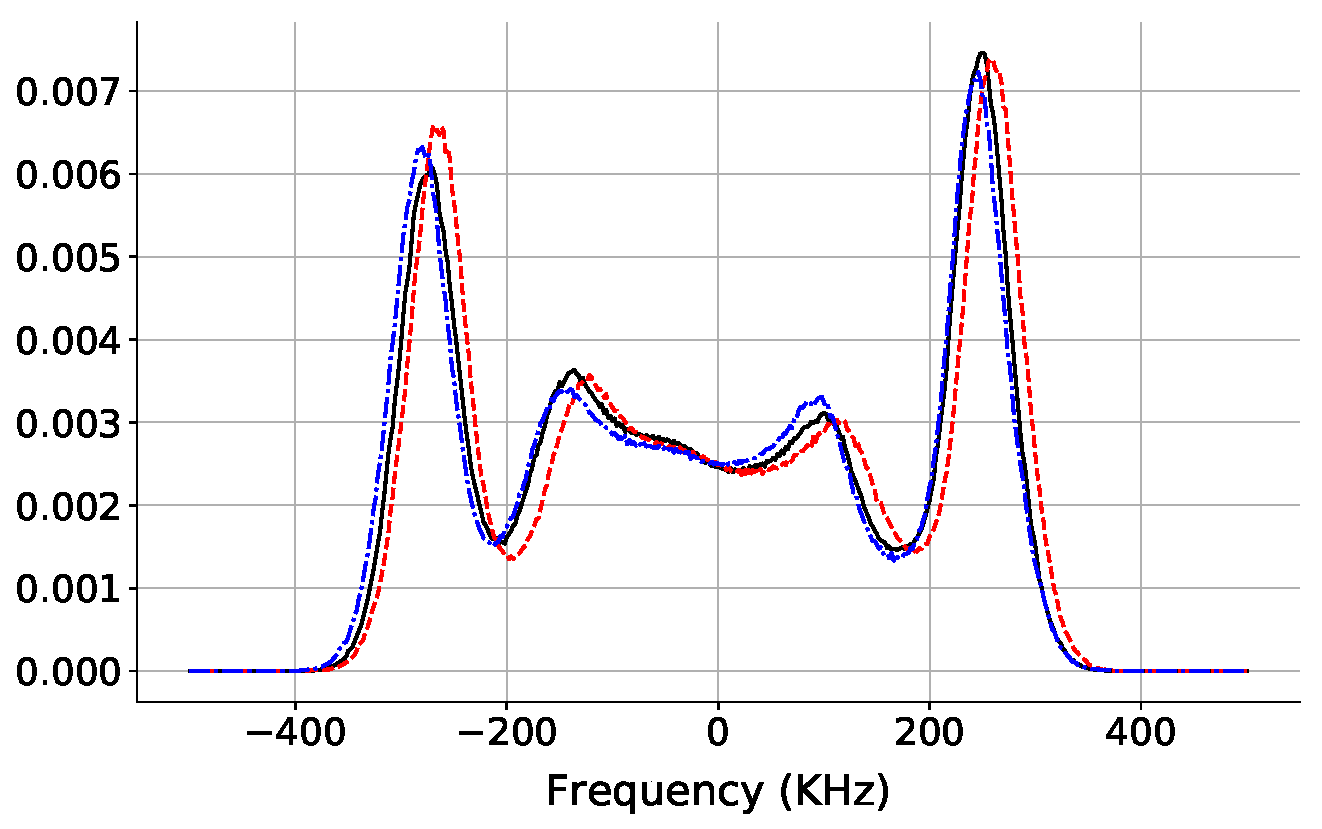
\includegraphics[width = \linewidth]{plots/Hist.pdf} 
\caption{The Histogram of 3 different CC2640 BLE chipsets, SNR = 30 dB}
\label{fig:3}
\end{figure}


%%%%%% Hadi: I have reviewed until here
\subsubsection{Environmental Effects}
\label{methodology:env}
To have a practical fingerprinting algorithm, it must be resistant to different environmental conditions. Therefore, we theoretically analyze the effect of different environmental condition on the histogram. In the evaluation section, extensive evaluations on the impact of different environmental conditions is presented. Moreover, field experiments are done to guarantee the practicality of the proposed fingerprinting methods in a real-world environment.

\paragraph{Coherence Time and Bandwidth} The delay spread in indoor environment is usually very small (e.g. 50 ns in homes). Thus, the coherence bandwidth is significantly larger than the bandwidth of BLE transmission (less than 1 MHz). As a result, frequency selective fading will not affect the frequency profile obtained by Histogram. On the other hand large scale fading and attenuation, will not affect the instantaneous frequency we obtain. Moreover, the fixed phase shift will be canceled as we use the temporal difference in phase to calculate the instantaneous frequency.
\begin{comment}
Multi-path effect does not drastically change between three consecutive samples. Therefore, three consecutive samples will have the same attenuation and phase shift due to the multi-path effect. As we just use the derivative of phase which is obtained by calculating numerical derivative using the next and previous sample, multi-path effect will not affect our instantaneous frequency measurement.
\end{comment}

Furthermore, this attack is practical in indoor environments rather than outdoor, due to the short communication range of BLE which makes it harder to receive in outdoor environments. Thus, the Doppler effect will not affect our algorithm since the transmitter will not move fast in indoor environment. Therefore, coherence time is significantly larger than the short transmission time of a BLE packet.
\begin{comment}
The Doppler shift for a device inside a car with $100 km/h$ speed is about $f_m = 222 Hz$ which is negligible compared with measurement resolution and errors. Also, the coherence time for such a scenario is about $T_C = \frac{9}{16 \pi f_m} = 8 ms$ which is greater than the packet time for BLE which is at most 3 ms and usually less than 1 ms. 
\end{comment}

\paragraph{Signal-to-Noise Ratio} To analyze the effect of noise, we consider the most common type of noise in communication systems , that is Additive White Gaussian Noise (AWGN). Due to the randomness of noise, the noise added to each sample is uncorrelated with that of other samples and thus, it could be different. As we measure the phase by using formula $tan^{-1}(\frac{Q}{I})$ where $I$ and $Q$ are in-phase and quadrature  part of the signal, each phase measurement will have an error due to noise. Since this error is different for each sample, we have an error in measuring instantaneous frequency. As the error in phase has a probabilistic nature, frequency measurement error also has a probabilistic nature. Let the frequency measurement error has a probability distribution $f$. We will argue that although each frequency measure has some random error due to noise, the effect of this random error on Histogram shape is deterministic and only dependent on the parameters of probability distribution $f$. As a result, utilizing Histogram as the input feature vector to learning model will make it easier for the model to ignore the noise effect.

%\todo{delete next two paragraphs or only retain the second paragraph}
Consider a random variable with the probability distribution $f$. 
%with $d$ parameters $p_1,p_2,p_3,...,p_d$. 
Assume we draw a set of $n$ samples $X=\{x_1,x_2,x_3,...,x_n\}$ and then another set of $n$ samples $Y=\{y_1,y_2,y_3,...,y_n\}$ from this distribution. Although the values of samples in these two sets are completely different with each other, their Histogram will be similar for large enough $n$ since Histogram represents the distribution of those sequence of samples which converges to $f$ as $n$ grows. This is the key insight behind how using Histogram as the feature vector can handle different noise levels. The random errors in measuring instantaneous frequency values will appear as a predictable shape in histogram given the parameters of the error in frequency measurements due to noise. Thus, the learning model will have an easier task to ignore the effect of noise. For example, assuming AWGN, these parameters only depend on SNR and as we show in Section~\ref{sec:results}, this technique performs well under different SNR values.

%Therefore, during the training, we employ data augmentation by adding artificial AWGN so that the learning model has enough data with various SNR values to learn how to estimate noise parameters and ignore noise effects. Fig. XXXXXX shows the histogram of an ideal (i.e. without hardware imperfection) 500 microsecond packet together with the histograms of a very long packet for 25dB SNR. As mentioned earlier, the histogram of a smaller set of samples approximately looks the same as the real distribution which is simulated by taking the histogram of a long packet. Fig. \todo{XXXXXX} shows how noise changes the histogram shape (or frequency distribution) of an ideal GFSK signal for different SNR values. The bin width of all histograms is 3 KHz. Finally, although we assumed the noise to be AWGN, one can argue the same analysis for other types of noise.


\begin{comment}
\subsubsection{Hardware Imperfection Effects}
In the rest of this section, we provide a detailed analysis on how different hardware imperfection represents themselves in the Frequency Distribution. This will prove our claim that our proposed methodology will retain all hardware imperfections while building a robust fingerprint.

\paragraph{Frequency Offset and Frequency Deviation} Ideally the histogram should have two peaks exactly at $\pm f_d$. However, carrier frequency offset caused by local oscillator may shift both peaks in the same direction as shown in Fig. XXXXXX. Moreover, the frequency deviation determines the frequency distance between two peaks which may not perfectly match the intended value and cause a reduction in the distance between two peaks as shown in Fig. XXXXXX. These two effect can even cause asymmetry in the position of the peaks. Also, the tail of the shape around one of the peaks, can slightly change the position of the other peak. 
\end{comment}

\begin{comment}
%%%%%%%IQ phase imbalance
\begin{figure}[t!]
 
\begin{subfigure}{0.5\textwidth}
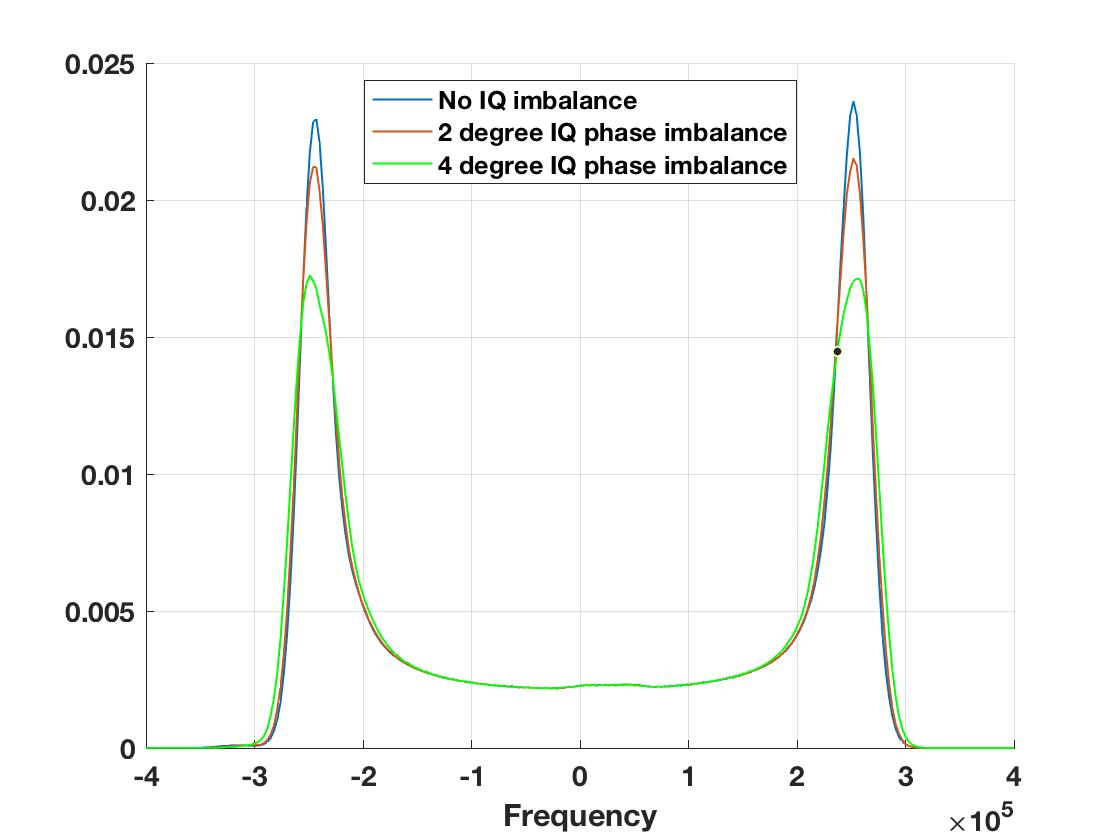
\includegraphics[width = 8cm, height=6cm,scale=0.5]{plots/00iq_phase_hist.jpg}
\caption{Effect of IQ phase imbalance on histogram}
\label{fig:iqphase}
\end{subfigure}
\begin{subfigure}{0.5\textwidth}
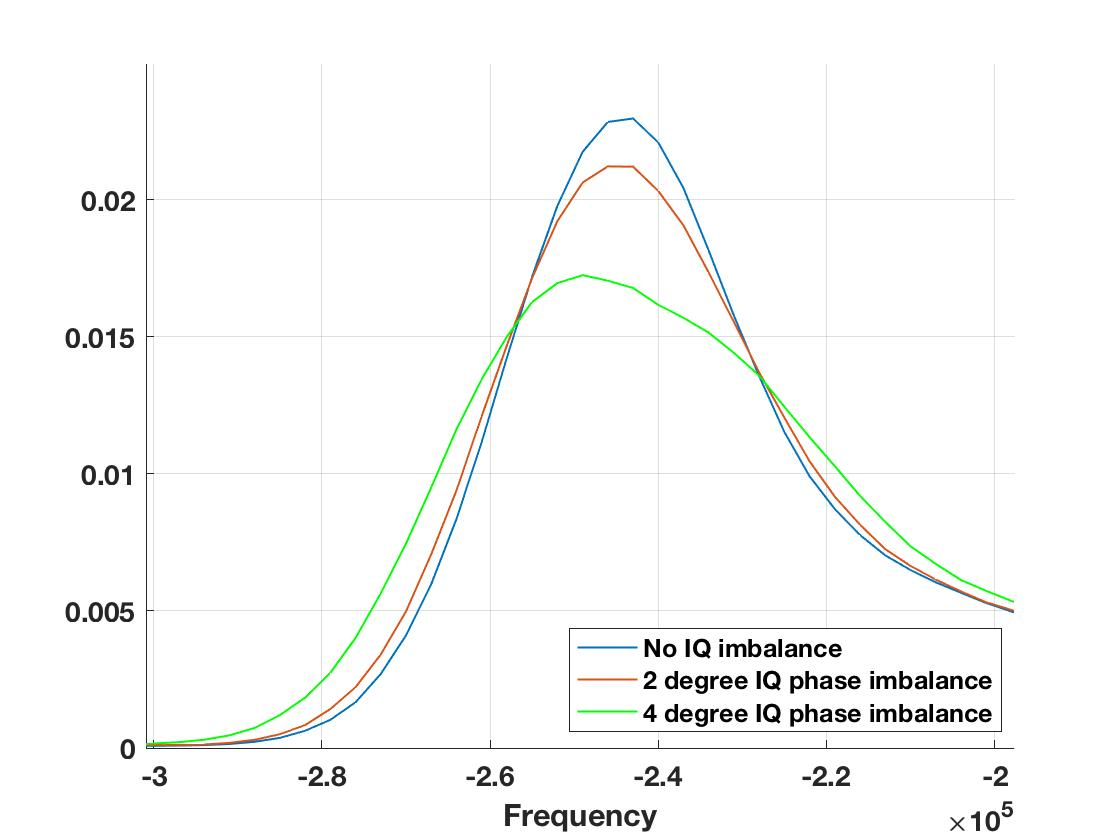
\includegraphics[width = 8cm, height=6cm,scale=0.5]{plots/00iq_phase_zoom_hist.jpg}
\caption{Effect of IQ phase imbalance on histogram - A closer look at one side}
\label{fig:iqphasezoom}
\end{subfigure}
 
\caption{Effects of IQ phase imbalance on histogram for different phase imbalance degrees}
\label{fig:7}
\end{figure}




%%%%%%%IQ amp imbalance
\begin{figure}[t!]
 
\begin{subfigure}{0.5\textwidth}
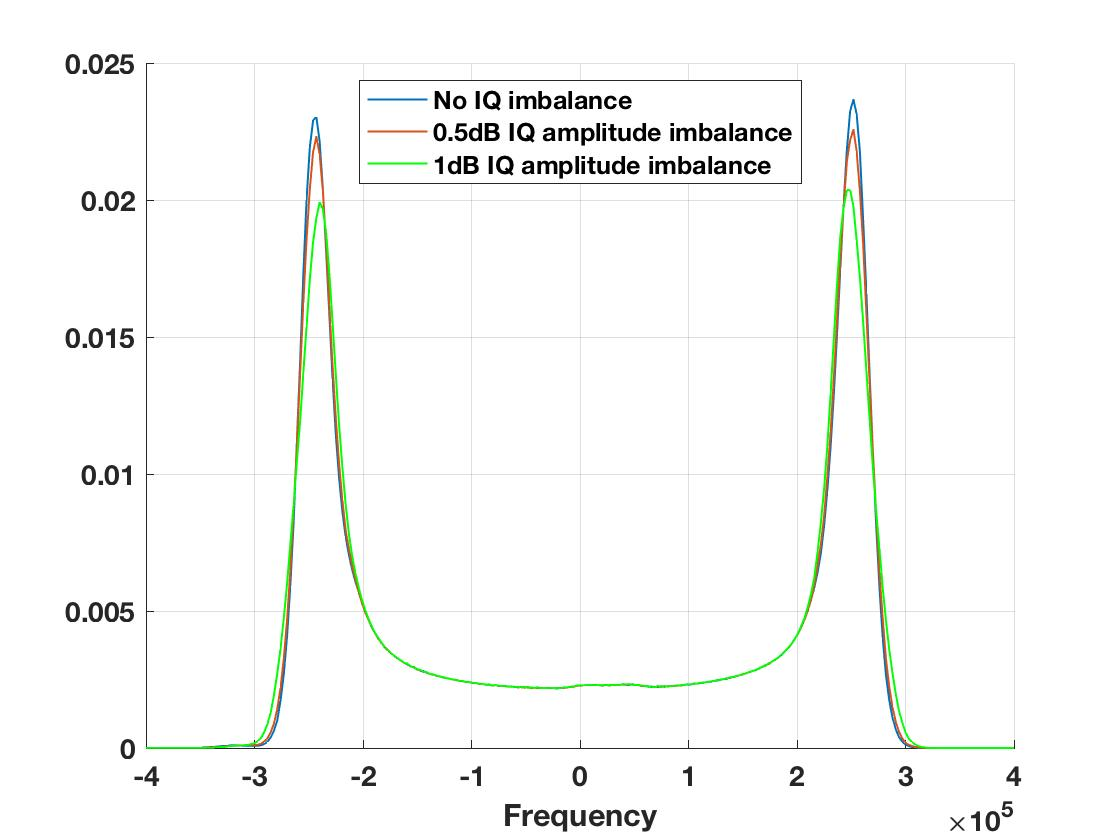
\includegraphics[width = 8cm, height=6cm,scale=0.5]{plots/00iq_amp_hist.jpg}
\caption{Effect of IQ amplitude imbalance on histogram}
\label{fig:iqamp}
\end{subfigure}
\begin{subfigure}{0.5\textwidth}
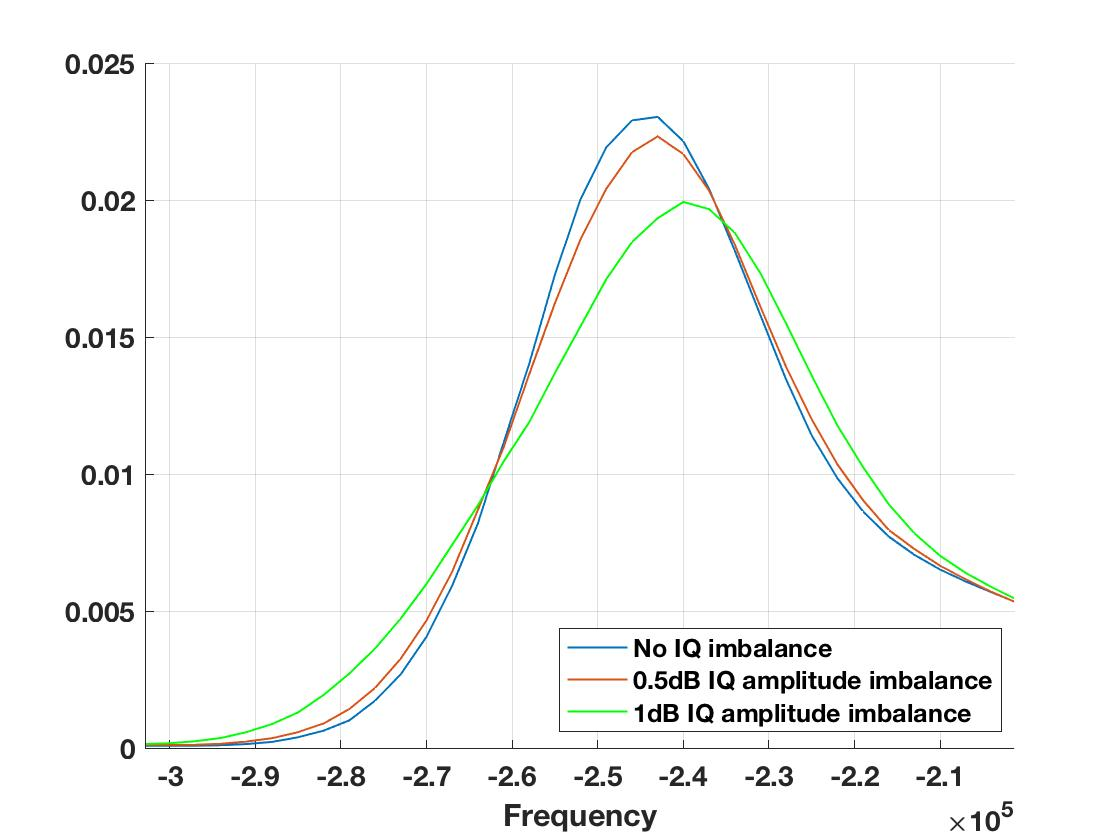
\includegraphics[width = 8cm, height=6cm,scale=0.5]{plots/00iq_amp_zoom_hist.jpg}
\caption{Effect of IQ amplitude imbalance on histogram - A closer look at one side}
\label{fig:iqampzoom}
\end{subfigure}
 
\caption{Effects of IQ amplitude imbalance on histogram for different amplitude imbalances}
\label{fig:8}
\end{figure}




%%%%%%%IQ offset
\begin{figure}[t!]
 
\begin{subfigure}{0.5\textwidth}
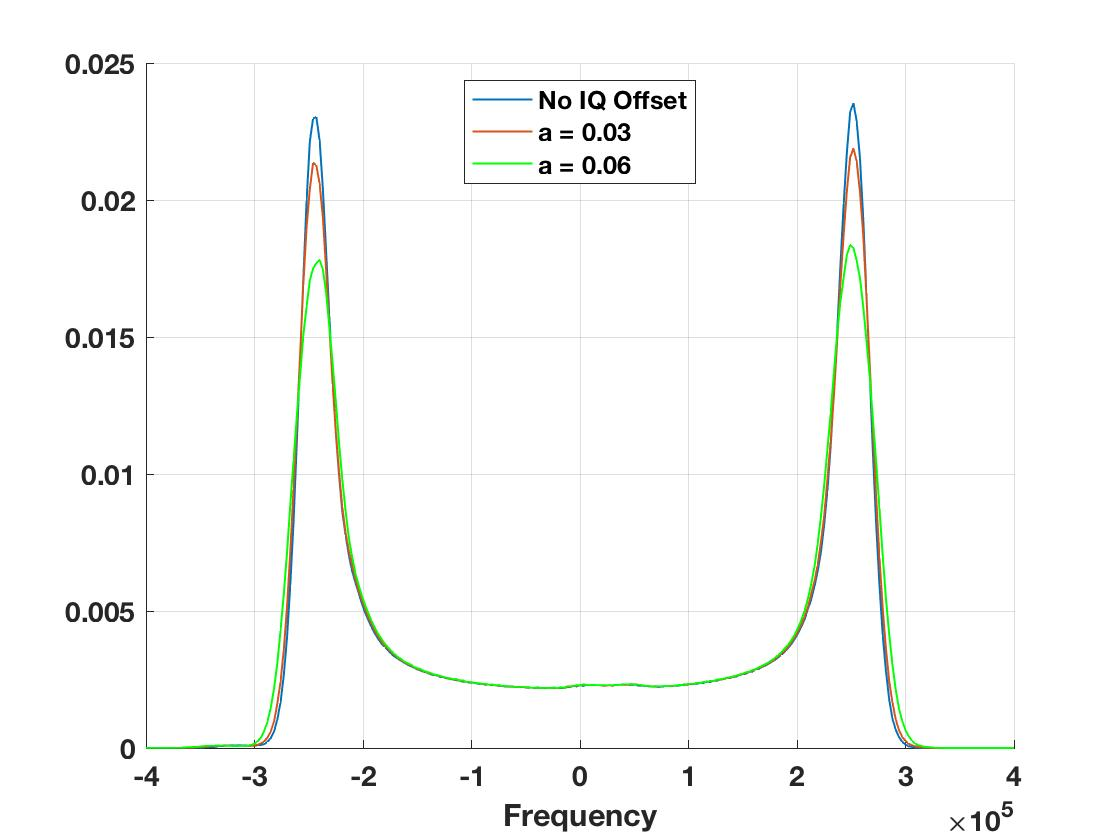
\includegraphics[width = 8cm, height=6cm,scale=0.5]{plots/00iq_offset_hist.jpg}
\caption{Effect of IQ offset on histogram}
\label{fig:iqoff}
\end{subfigure}
\begin{subfigure}{0.5\textwidth}
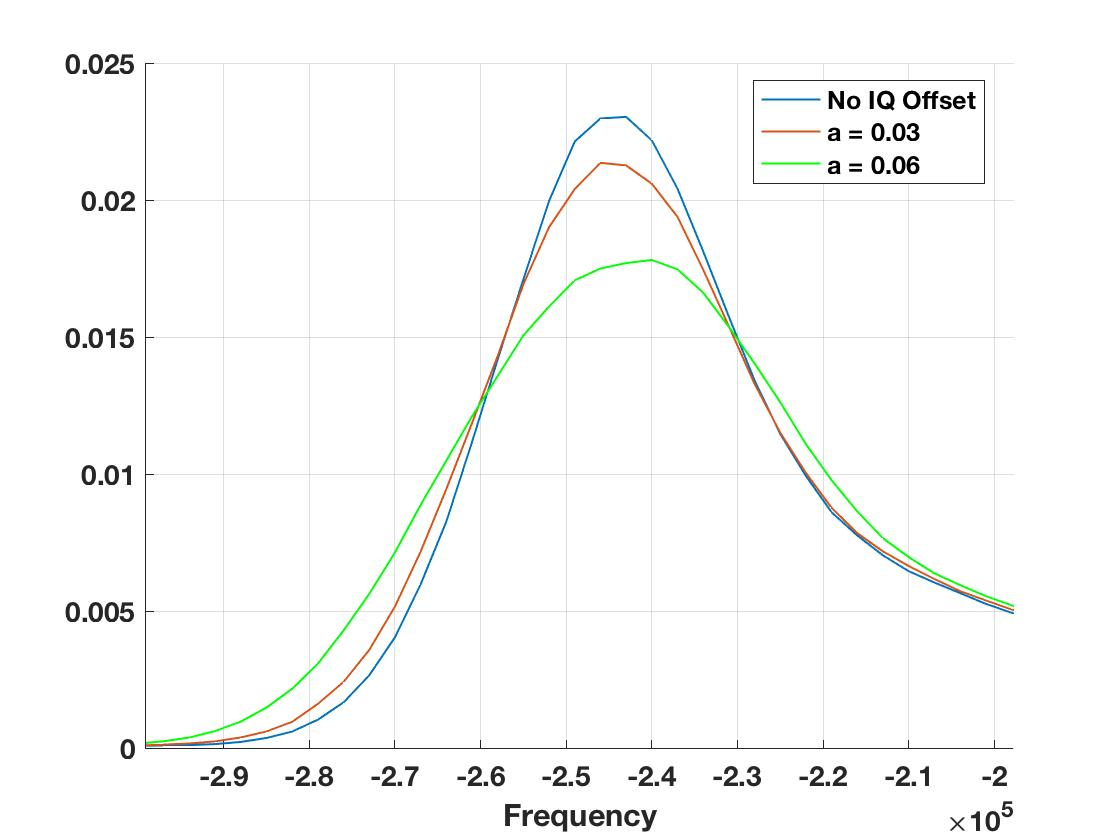
\includegraphics[width = 8cm, height=6cm,scale=0.5]{plots/00iq_offset_zoom_hist.jpg}
\caption{Effect of IQ offset on histogram - A closer look at one side}
\label{fig:iqoffzoom}
\end{subfigure}
 
\caption{Effects of IQ offset on histogram for different offset magnitudes}
\label{fig:9}
\end{figure}

\subsubsection{I/Q Imbalance}
The ideal IQ components (normalized in amplitude) of the GFSK signal are $I+jQ = cos(2\pi ft)+jsin(2\pi ft)$ where $f$ is the frequency of the signal. However, if due to the mismatch between I and Q path, the ratio of the Q amplitude to I amplitude is $a$ and their phase difference is $\phi$, then we have $I'+jQ' = cos(2\pi ft)+jasin(2\pi ft+\phi)$. Therefore, the phase of the signal will be $tan^{-1}(\frac{Q}{I})=tan^{-1}(\frac{asin(2\pi ft+\phi)}{cos(2\pi ft)})$. For the sake of simplicity, we assume the frequency does not change fast between 2 consecutive samples while calculating numerical derivative of phase (that is, the frequency is independent of time which is true only when frequency is stable at bit 0 or 1 in GFSK). Removing this assumption will not change the end conclusion. The frequency of the signal at time $t$ will be

%\begin{equation}
\begin{gather*}
    \frac{d}{dt}tan^{-1}(\frac{asin(2\pi ft+\phi)}{cos(2\pi ft)}) \\= 
    2\pi f \frac{acos(\phi)}{a^2sin^2(2\pi ft+\phi)+cos^2(2\pi ft)}
\end{gather*}
%\end{equation}
whereas ideally, it should be $2\pi f$. This imperfection will be reflected in histogram as shown in Fig. \ref{fig:7} for phase imbalance ($a = 1$) and Fig. \ref{fig:8} for amplitude imbalance ($\phi=0$).


\subsubsection{I/Q Offset}
IQ origin offset can be modeled as 
%\begin{equation}
\begin{gather*}
    I'+jQ' = e^{2 \pi ft}+ae^{j\phi} \\= 
    cos(2\pi ft)+acos(\pi) +j(sin(2\pi ft)+asin(\pi)) \\= cos(2\pi ft)+i +j(sin(2\pi ft)+q)
\end{gather*}
%\end{equation}
where $q = acos(\pi)$ and $i = asin(\pi)$. The frequency of the signal with IQ offset at time $t$ will be

%\begin{equation}
\begin{gather*}
    \frac{d}{dt}tan^{-1}(\frac{sin(2\pi ft)+q}{cos(2\pi ft)+i}) = \\ 2\pi f \frac{sin(2\pi ft)\big( sin(2\pi ft)+q \big)+cos(2\pi ft)\big( cos(2\pi ft)+i \big)}{\big( sin(2\pi ft)+q \big)^2+\big( cos(2\pi ft)+i \big)^2}
\end{gather*}
%\end{equation}
whereas ideally, it should be $2\pi f$. IQ origin offset imperfection effects on histogram is shown in Fig. \ref{fig:9} for $\phi = \frac{\pi}{4}$ and different values of $a$.
\end{comment}
\begin{comment}
\paragraph{PLL Imperfection} As there is no IQ paths and mixer and samples are directly passed to PLL in the aforementioned low power architecture, the instantaneous frequency will have the information about imperfections in the PLL. These information can originate for different reasons. Since the histogram is profiling instantaneous frequency, it will include these information as well.

\paragraph{Transient} Transient portion of a signal is transmitted upon power-up stage of the transmitter during which capacitive loads charge and the power amplifier ramps its power output. As during this stage, the frequency is equal to carrier frequency, transient portion of the signal will appear as another peak in the middle of the histogram (that is, at frequency 0 KHz if there is no CFO and other imperfections).
\end{comment}
%\subsubsection{Gaussian Filter}

\begin{comment}
IQ offset can be modeled as a vector $I'+jQ' = A'e^{j\phi'}$ added to the original IQ samples $I+jQ = Ae^{j\phi(t)}$:
\begin{gather*}
    I+jQ+I'+jQ' = Ae^{j\phi(t)}+A'e^{j\phi'}
\end{gather*}

when there exists a CFO of $\Delta f$, it will change the phase of IQ offset as follows:
\begin{gather*}
    (Ae^{j\phi(t)}+A'e^{j\phi'})\times e^{j2\pi \Delta f t} \rightarrow IQ_{offset} = A'e^{j(\phi'+2\pi \Delta f t)}
\end{gather*}
Therefore, the vector by which we represent IQ offset is changing as the time changes which means for each time instance we have a different IQ offset. For example, for a packet of length 100 microseconds and CFO of just 1KHz, the phase of IQ offset will change by 36 degree from the start to the end of packet.
\end{comment}


\subsection{Putting it all together}


The first step in deploying our RF fingeprinting attack is to capture the BLE signal. We use SparSDR~\cite{?}, as it capture entire ISM bandwidth, and also minimizes the size of captured data as it only captures I and Q samples of the data when there is an actual transmission. Next, we use the captured signal to fingerprint the device. The entire processing flow can be divided into two stages, Fingerprinting Stage and Identification Stage. In the former stage, we train the machine learning models to classify devices based on their RF fingerprints. This stage happens when the MAC address of the device is fixed during a MAC address lifetime and we can have the groundtruth (labels) for training. The latter stage, employs the trained models to identify different devices when their MAC addresses have changed.


\paragraph{Fingerprinting Stage} In order to fingerprint all BLE devices, we combine both gradient descent based CFO and IQ imperfection estimation which is sufficient to distinguish combo transmitters and Histogram which is sufficient to distinguish BLE-only transmitters together with CFO. CFO anf IQ imperfections can be extracted with a high resolution using algorithm described in~\ref{sec:methodology1}. However, 1000-dimension Histograms need to be further processed to reduce the dimensionality. Conventional dimensionality reduction algorithms such as PCA might be used. However, we found that because of the significant change in the shape of Histogram caused by SNR variation, PCA cannot significantly reduce the dimensionality while preserving the necessary information. Due to the same reason, distribtuion similarity metrics such as KL-divergence cannot be directly applied to measure the similarity between two Histograms. Among all traditional methods that we experimented, we observed that fitting Gaussian Mixture Models (GMM) to the histograms together with hand-crafted statistics, can result in a decent performance. However, since low SNR affects both means and variances extracted by GMM, the performance degrades when SNR is not high.

Its worth mentioning that although SNR will change the shape of Histograms, this change is similar for the same SNR values as discussed in~\ref{methodology:env} (note that if we used the raw I/Q samples, noise would change the signal randomly even for the same SNR value. This would make it hard for learning-based or hand-crafted algorithms to perform well under low SNR condition as prior RF fingerprint works mostly fail in low SNR regime). As a result, we need to have a technique that captures how different SNR levels change Histograms, ignores those effects, preserves necessary information for classifying Histograms of different devices, and finally reduces the high dimensionality of Histogram. Convolutional neural networks (CNN) is a natural fit to achieve these goals as they can learn to deal with different SNR levels and maintain necessary information that distinguishes different classes. Therefore, to extract features from the Histogram and reduce its dimenwionality, we employ a CNN with 3 convolutional layers followed by a fully connected layer, and a classifier. We did not observe significant improvements by adding more layers probably because of the simple shape of Histograms. We first train the network on the training data with a softmax classifier at the end and cross entropy loss function. Then we remove the classifier layer and use the resulting network as a feature extractor. This feature extractor will be used to extract features from new Histogram during the test (identification stage).

We call the 16 deimensional feature vector extracted from a Histogram $F_1$.  Then we obtain CFO, IQ offset and IQ imbalance by gradient descent method and call the resulting feature vector $F_2$. We train a support vector machine (SVM) with RBF kernel on the resulting $\{F_1,F_2\}$ feature vector. The reason for choosing SVM as the ultimate classifier is having the flexibility to learn sufficiently tight boundaries around the targets and classify outliers as non-target devices in order to decrease false positive rate. Several other classifier might be used and yield competitive accuracies but we saw the best performance when having sufficiently tight boundaries around the targets. Comparing the performance of different classifiers is out of the interest of this paper.


%Note that IQ offset and imbalance are only useful for combo transmitters and will be ignored by classifier while classifying BLE-only transmitters.
\paragraph{Identification Stage}
To identify a device, we obtain $F_1$ by using the CNN feature extractor, and $F_2$ by using the gradient descent. Then, $\{F_1,F_2\}$ feature vector will be classified by the SVM to identify the device. The design of the classifier is illustrated in Figure~\ref{fig:alg}. The detail of training and testing the model is discussed in the next section. 

\begin{figure}[t!]
    \centering
    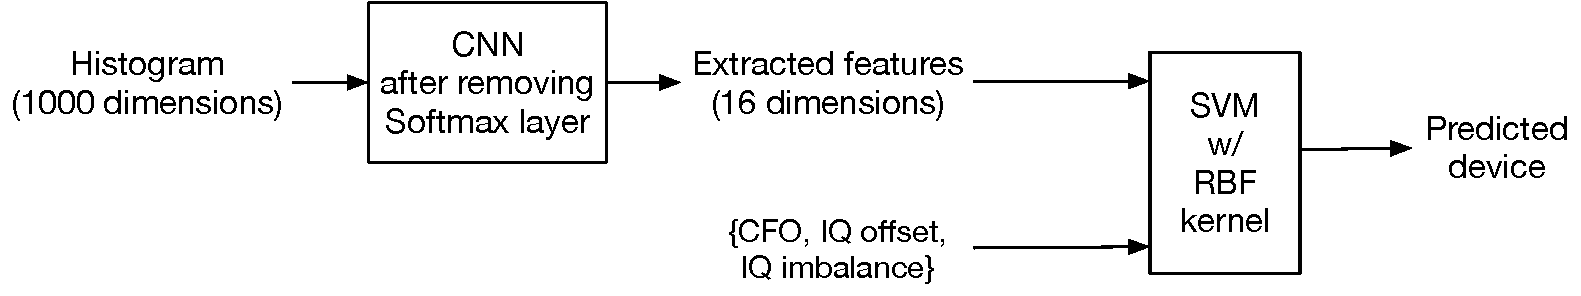
\includegraphics[width = \linewidth]{plots/algorithm_flow.pdf} 
    \caption{Identification Stage}
    \label{fig:alg}
\end{figure}


\begin{comment}
\begin{figure}[t!]
    \centering
    \includegraphics[width = \linewidth]{plots/CNN2.pdf}
    \caption{CNN architecture}
    \label{fig:10}
\end{figure}
\end{comment}

%\subsection{System Design}


\begin{comment}
Although classical machine learning algorithms such as principal component analysis (PCA) or fitting Gaussian Mixture Model (3 Gaussian corresponding to two peaks around frequency deviation and one peak corresponding to transient) to raw instantaneous frequency measurements and feeding the resulting means and variances to an ensemble of trees to as a classifier, produces decent classification accuracy, it does not capture all the information. For instance, intuitively Gaussian Mixture Model (GMM) does not capture the effects of IQ imbalance and IQ offset completely. As a result, we feed histogram as the input feature vector to convolutional neural networks (CNN) which are well-known for capturing shapes. The network is constructed from 3 convolutional layer and 3 fully connected layer, followed by a softmax classifier. We used Nesterov Adam optimizer and cross entropy loss function. The details of the network is shown in Fig. \href{fig:10}.



\begin{figure}[t!]
\centering
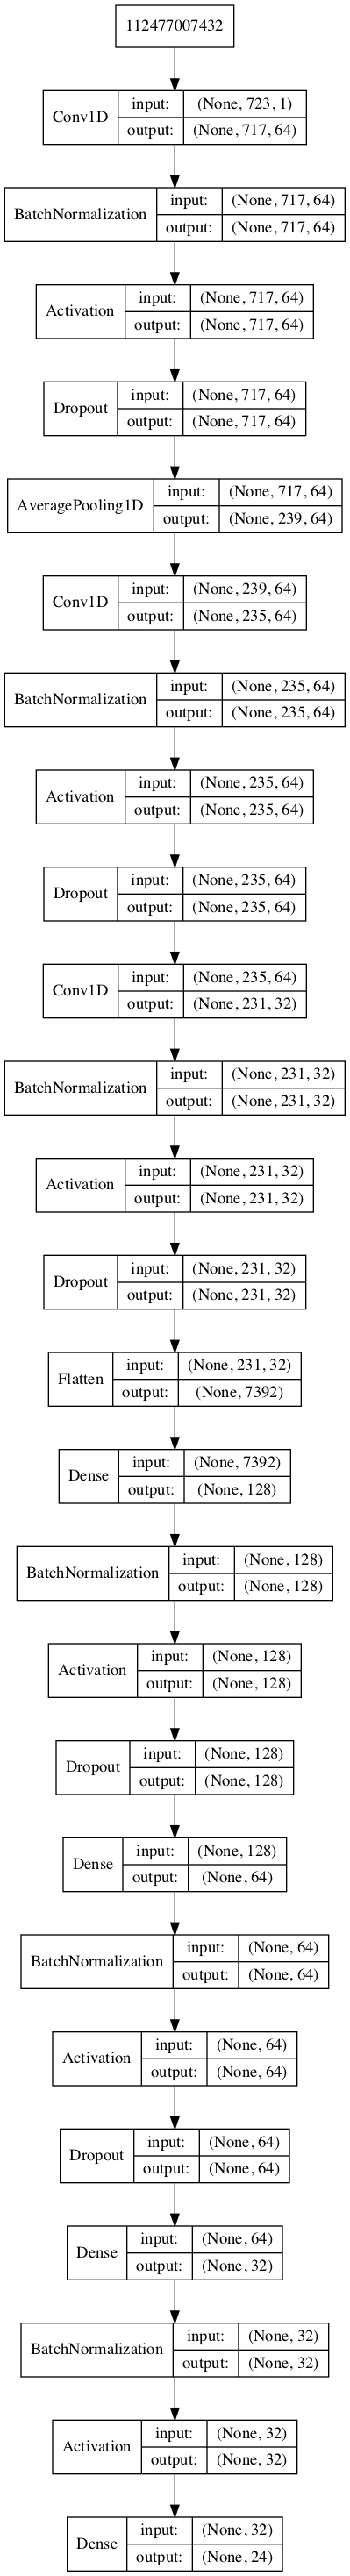
\includegraphics[width = 4cm, height=20cm,scale=0.5]{plots/model.png}
\caption{CNN structure}
\label{fig:10}
\end{figure}
%\subsubsection{Classical Machine Learning}

%\subsubsection{Deep Learning}


%\subsection{Attack Model}
%The goal of attack is detecting the presence of someone around the attacker. However, one can employ multiple receivers and compensate for the receivers' hardware imperfection in order to make tracking attack possible. As mentioned earlier, BLE suggest MAC address randomization after 15 minutes and most of the popular devices randomize their MAC address after 15 minutes or more. We call this period in which the MAC address of a device is fixed, a "Slot". The attacker receives packets during the first slot from a device. Since the MAC address is fixed during that slot, it can label all those packets as the same transmitter. The attacker 
\begin{figure*}[t!]
\centering
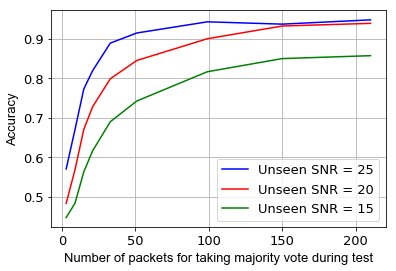
\includegraphics[width = 13cm, height=8cm,scale=0.5]{plots/00ac.png}
\caption{Classification accuracy of 20 BLE devices using CNN vs Number of packets used for majority vote during test- "Unseen SNR" means the SNR value of test set - SNR value of test set was not used in any packet in training set}
\label{fig:11}
\end{figure*}

\end{comment}